\documentclass[11pt,a4paper]{article}

\usepackage{main}
\usepackage{cours}

\renewcommand{\typedocument}{Cours}
\renewcommand{\classe}{6e}
\renewcommand{\titre}{Energie}

\begin{document}

\pagination

\creertitre{Energie}

\partie{Introduction}

Au quotidien, nous utilisons de l'énergie pour vivre. Nous nous en servons pour:
\begin{itemize}
    \item nous déplacer,
    \item faire fonctionner notre corps humain,
    \item nous éclairer,
    \item nous chauffer,
    \item faire fonctionner nos appareils électriques.
\end{itemize}

\important{L'énergie est une grandeur physique, son symbole est $E$ et son unité est le joule ($J$).}

Mais d'où viennent toutes ces énergies dont nous avons besoin ? On ne peut pas créer de l'énergie à partir de rien, il faut la transformer à partir d'une autre forme d'énergie.

\partie{Les six formes d'énergie}

Lorsqu'un objet est en mouvement, il possède de l’\important{énergie mécanique}.

Le soleil produit de la lumière (\important{énergie lumineuse}) et de la chaleur (\important{énergie thermique}).

Pour faire fonctionner notre corps, on mange des aliments. Notre système digestif les transforme avec des réactions chimiques. Les aliments fournissent de l’\important{énergie chimique}.
Tout ce qui peut faire des réactions chimiques (pile, batterie, combustible) contient de l’énergie chimique.

Les appareils ménagers (four, ordinateur) utilisent de l’\important{énergie électrique}.

Dans les centrales nucléaires, on utilise de l’Uranium qui fait des réactions nucléaires : il contient de l’\important{énergie nucléaire}.

L'énergie mécanique, lumineuse, thermique, chimique, électrique et nucléaire sont les six formes d'énergie.

\partie{Conversion d'énergie}

\souspartie{Principes de base}

En introduction, nous avons vu la loi suivante :

\vspace{15pt}

\fbox{\parbox{\textwidth}{%
\important{Principe 1:} L'énergie ne peut pas être créée ni détruite, elle peut seulement être transformée d'une forme en une autre.
}}

\vspace{15pt}

On appelle \important{conversion d'énergie} la transformation d'une forme d'énergie en une autre.

On appelle \important{convertisseur} d'énergie le système qui permet de faire une conversion d'énergie.

On peut représenter les conversions d'énergie à l'aide de \important{schémas de chaîne d'énergie}:

\begin{itemize}
    \item les convertisseurs d'énergie sont représentés par des rectangles,
    \item les formes d'énergie sont représentées par des flèches
\end{itemize}

\newpage

\exemple{Un moteur de voiture transforme de l'énergie chimique (carburant) en énergie mécanique (mouvement de la voiture), mais le moteur chauffe, une partie de l'énergie est perdue sous forme d'énergie thermique (chaleur).}

\begin{center}
    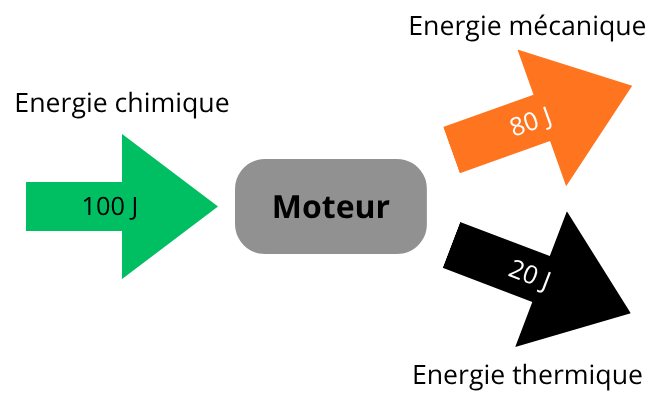
\includegraphics[width=9cm]{images/moteur.png}    
\end{center}

Lors d'une conversion, l'énergie se conserve. C'est une autre loi à retenir :

\vspace{15pt}

\fbox{\parbox{\textwidth}{%
\important{Principe 2:} Il y a autant d'énergie à la fin de la conversion qu'au début. C'est le principe de conservation de l'énergie.
}}

\vspace{15pt}

Parfois, de l'énergie est perdue lors d'une conversion, mais elle n'est pas détruite, elle est simplement transformée en une forme d'énergie que nous ne pouvons pas utiliser.

\newpage

\partie{Sources d'énergie}

Autour de nous se trouvent de nombreuses \important{sources d'énergie}.

Certaines sont \important{renouvelables} (il y en a une quantité illimitée ou elles se régénèrent rapidement à l'échelle humaine):
\begin{itemize}
    \item le soleil (utilisé par les panneaux solaires),
    \item le vent (utilisé par les éoliennes),
    \item l'eau (utilisée par les barrages hydroliques).
\end{itemize}

Mais d'autres sont \important{non renouvelables}, si on les utilise, elles s'épuisent et ne se régénèrent pas assez rapidement à l'échelle humaine:
\begin{itemize}
    \item l'uranium (utilisé par les centrales nucléaires),
    \item les énergies fossiles : pétrole, charbon, gaz naturel (utilisées par les centrales thermiques). Ces sources d'énergie sont très polluantes.
\end{itemize}

Les humains ont principalement besoin d'énergie électrique mais ces sources d'énergie sont sous des formes différentes.

Il faut donc faire des conversions d'énergie pour les transformer en énergie électrique.

\exemple{Le soleil fournit de l'énergie lumineuse. Pour exploiter cette énergie, on utilise des panneaux solaires qui convertissent l'énergie lumineuse en énergie électrique. Lors de la conversion, une partie de l'énergie est perdue sous forme d'énergie thermique.}

\begin{center}
    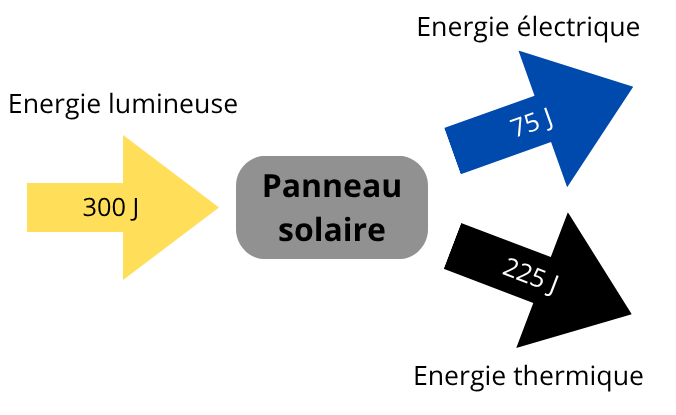
\includegraphics[width=9cm]{images/pv.png}
\end{center}

\end{document}